%God give me strenght
\chapter{Úvod}

Historické texty nám ukazujú, že človek mal vždy tendenciu si informácie ukladať - zapisovať. Či sa jednalo o písanie na steny v jaskyniach, papyrusové zvytky alebo tlačené knihy. V priebehu času sa vyvíjali materiály aj technológia, ktorou tieto informácie zapisujeme. Hoci už sme v 21. storočí a pomaly každý z nás vlastní nejaké smart zariadenie stále využívame pero a papier na poznámky, písanie poštovej korešpondencie a aj ako spôsob našej identifikácie - podpisovanie. Podpis stále hraje neodmysliteľnú úlohu pri dávaní súhlasu s úradnými dokumentami, autorstvom dokumentov a overovaní identity osôb. Práve pre jeho používanie v úradných dokumentoch sa častokrát stáva terčom falšovania.

Cieľom tejto práce bude vytvoriť zariadenie schopné zaznamenávať dynamické vlastnosti písma pomocou senzorov ukrytých vo vnútri pera. 

V druhej kapitole sa rozoberajú existujúce riešenia pier s rôznymi typmi senzorov spolu s teoretickým základom k dynamickým vlastnostiam písma. V tretej kapitole sa náchadza návrh konštrukcie pera so skrytými senzormi a výber jednotlivých komponent. Štvrtá kapitola obsahuje praktické riešenie návrhu a testovanie vytvoreného zariadenia. Piata kapitola zhrnie zistenia, ku ktorým sa prišlo pri testovaní.

\chapter{Teoretická část}

\section{Vlastnosti písania}

V tejto časti popíšem aké dáta chceme merať z písma.

\section{Existující technologie}

\subsection*{Livescribe 3}

Livescribe 3 je určené na písanie poznámok. Toto pero využíva Bluetooth v4.0 na spojenie s mobilným zariadením, do ktorého následne odosiela dáta o pohybe. Systém tieto dáta v reálnom čase prevádza do písaného textu, pričom je možné použiť aj funkciu konvertovania písaného textu do tlačenej podoby pomocou OCR (z anglického Optical Character Recognition Optické, česky rozpoznávání znaků. Na záznam pohybu využíva infračervenú kameru, ktorá sa nachádza na spodnej časti pera pod hrotom tuhy. Okrem písma zaznamenáva aj zvuk a tak písmo doplňuje ďalší kontext. Veľkosťou je sa jedná o kompaktné zariadenie - 162x14.9 mm a hmotnosťou 34 gramov.\newline

\subsection*{iskn Slate 2+}

Slate 2+ od firmy iskn využíva magnetický prstenec a špeciálnu podložku, v ktorej sa nachádza 32 magnetometrov (senzorov na meranie zmien magnetického poľa). Podložka komunikuje s aplikáciou v mobilnom zariadení alebo počítači pomocou Bluetooth LE v5.0 a v reálnom čase tieto dáta zobrazuje. Výsledok je veľmi presný, no vyžaduje presnú kalibráciu. Kalibrácia sa vykonáva tak, že sa na podložke stisne drží špeciálne tlačidlo a potom stačí vziať pero/ceruzku s prtencom a priložiť jej hrot kolmo na podložku. Následne stačí pustiť tlačidlo a všetko je nakalibrované. Ak sa kalibrácia nevykoná správne ceruzka nebude presná.\newline

\begin{figure}[hbt]
	\centering
	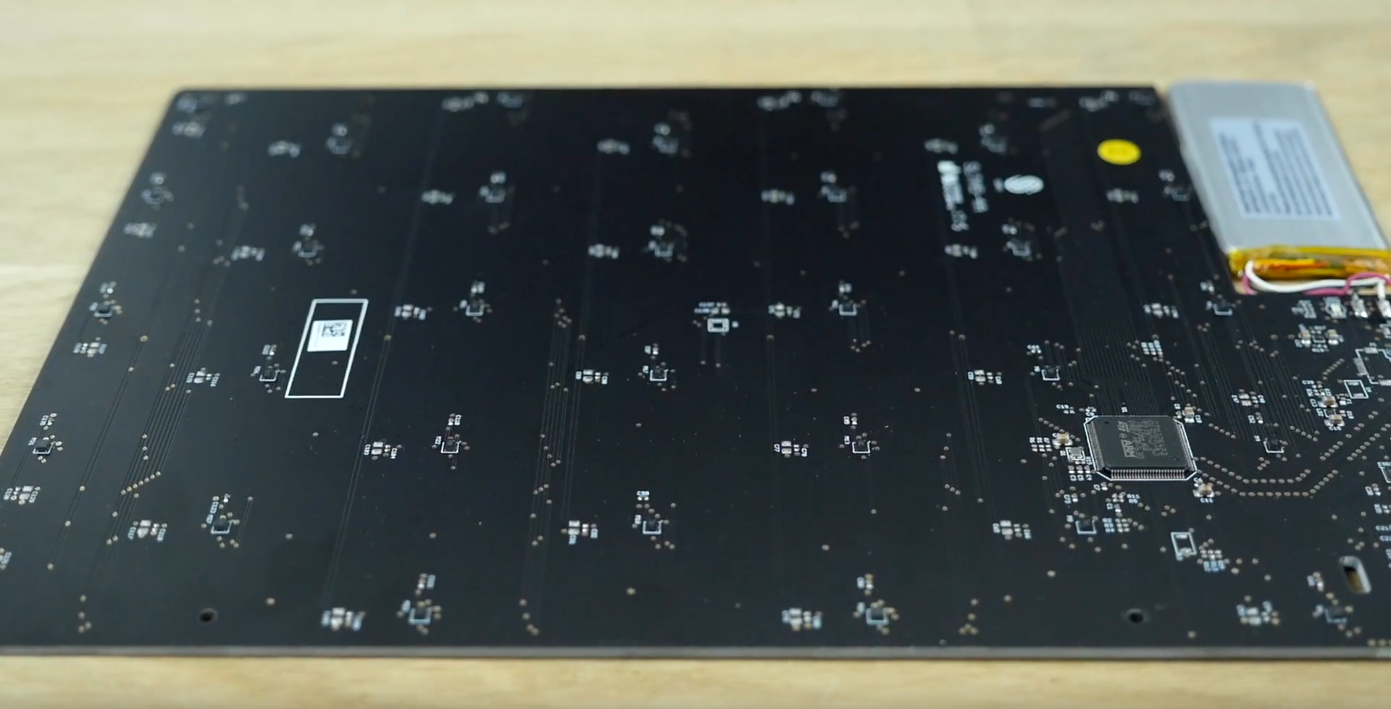
\includegraphics[width=0.5\textwidth]{obrazky-figures/isknBoard.png}
	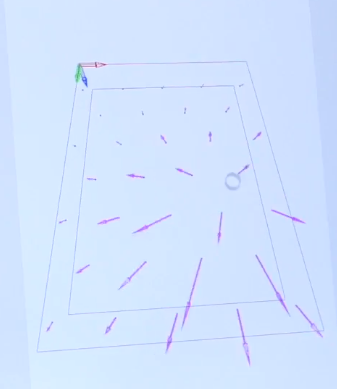
\includegraphics[width=0.3\textwidth]{obrazky-figures/isknMagneticfield.png}
	\caption{Board with sensors (left) and detected field (right)}
	\label{ISKN}
\end{figure}
%isknMagneticfield

\subsection*{Stylus}

Stylus sa používa na písanie na dotykové plochy. Aktuálne asi najsofistikovanejším je Apple Pencil. Radí sa mezdi aktívne stylusy\cite{HarleyJonahA2013As}. Používa dva trojosé gyroskopy rozmiestnené v rôznych častiach pera. Hrot pera funguje ako tlakový senzor a taktiež ako anténa, ktorá vysiela nízkofrekvenčné (dlhé) vlny a tie sú detekované senzorovou vrstvou pod displejom. Spojenie s iPadom zabezpečuje Bluetooth 4.1\cite{ApplePencilForum}. Intel v roku 2014 predpovedal, že aktívne stylusy nebudú také úspešné ako pasívne z dôvodu vysokej ceny a náročnosti vývoja takej technológie\cite{IntelDisp}. No ako môžeme vidieť, táto technológia nakoniec prerazila.\newline

\subsection*{Špeciálne výskumné perá}

Pri výskume zameranom na tlak pôsobiaci na hrot pri písaní sa používali dva analógové piezoelektrické biomorfné senzory prichytené na tuhu v 90\degree~uhle k sebe navzájom\cite{EernisseE}, viď obrázok X.X. Tento typ senzoru využíva piezoelektrických javov pri meraní pohybu pera. Iný výskum sa zaoberal identifikáciou pisateľa podľa tlaku, ktorý vyvíja na podložku, viac informácií v \cite{SchomakerL.1990Trbp}. V tomto výskume bol použitý tenzometer, pasivní elektrotechnická součástka, používaná jako senzor k nepřímému měření mechanického napětí na povrchu součásti prostřednictvím měření její deformace\cite{Tenzometr}.

\begin{figure}[hbt]
	\centering
	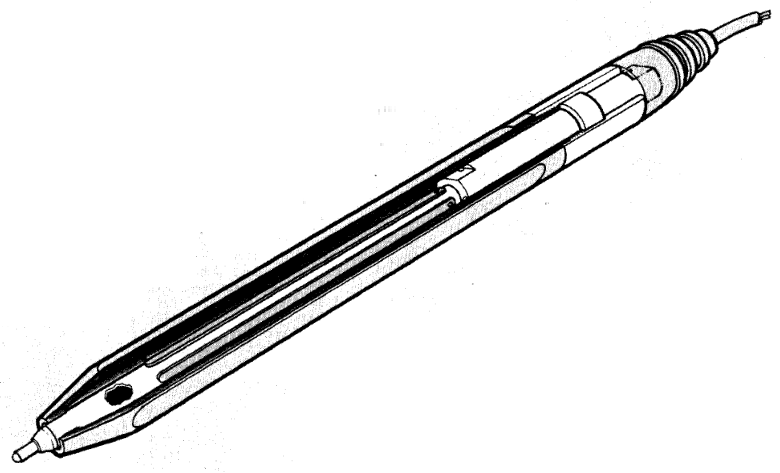
\includegraphics[width=0.3\textwidth]{obrazky-figures/piezoPen1997.png}
	\caption{Piezoelektrické pero}
	\label{piezoPen1997}
\end{figure}

\chapter{Návrh řešení}

V tejto časti sa budem venovať výberu komponent a samotnému návrhu pera so senzormi.

\section{Vlastnosti písma}

Pre návrh pera je nevyhnutné stanoviť si aké vlastnosti písma budem potrebovať zaznamenávať. 

\section{Stanovenie vlastností}

Z exitujúcich technických riešení me sa rozhodli niektoré vybrať a použiť ich pri návrhu a konštrukcii pera so skrytými senzormi. Ako názov tejto práce napovedá "Konstrukce pera se skrytými senzory" budeme chcieť vyrobiť pero, ktoré na prvý pohľad bude vyzerať nenápadne, tak aby si pisateľ nič podozrivé nevšimol. Z dôvodu ušetrenia miesta v zariadení bude najlepšie vytvoriť vlastný hardware, ktorý bude prepojovať mikrokontrolér so senzormi a zmestí sa do pera. Z technických dôvodov a mojej neskúsenosti budeme postupovať v niekoľkých iteráciách prototypov. Najprv budeme využívať už existujúce vývojové dosky a kity. V neskorších štádiách sa budeme venovať aj návrhu vlastného hardware. 

Infračervená kamera je asi najlepšie riešenie, čo sa týka presnosti, no rozhodli sme sa ju nepoužiť, pretože je príliš nápadná na to, aby si ju človek nevšimol. Nevylučujeme však, že by sa dala použiť a schovať na spodnú časť pera pod hrot tuhy, tak aby si to človek nevšimol, no pre tento výskum s ňou nebudeme počítať a prenechávame túto možnosť na ďalší výskum.

Kalibrácia je veľmi dôležitým parametrom keďže chceme aby bolo zariadenie presné, ale nie za cenu náročnej procedúry pri spúšťaní pera. Cieľom bude vybrať súčiastky tak, aby na kalibráciu stačilo minimum času. 

Rozhodli sme sa, že pero nesmie vyžadovať žiadnu špeciálnu podložku na záznam pohybu. Toto riešenie by vyžadovalo, aby sa človek podpísal na konkrétnu podložku. Hoci je pravdepodobne možné človeka zmanipulovať na to aby sa podpísal na konkrétnu plochu poprípade vytvoriť plochu povedzme veľkosti stola, rozhodli sme sa neísť touto cestou a pokúsime sa vytvoriť riešenie, ktoré nebude potrebovať dodatočný hardware. \newline

\textbf{Cieľové vlastnosti, na ktoré by sme sa chceli zamerať sú:}
\begin{description}
	\item[-]{presnosť}
	\item[-]{minimálna poprípade rýchla kalibrácia}
	\item[-]{skrytosť a nenápadnosť}
	\item[-]{možnosť písať na akomkoľvek povrchu}
\end{description}

Podľa týchto vlastností sme sa zamerali na výber vhosných komponet.

\section{Výber komponent}

\subsection*{Tlakový senzor}

Interlink Electronics FSR® 400 je malý a lacný tlakový odporový senzor. Bez záťaže sa správa ako nekonečný odpor a s použitím sily na jeho povrch sa jeho odpor znižuje. Citlivosť a~maximálna záťaž je nastavená na interakciu s ľuďmi. \cite{fsr400} V kombinácii s 10K Ohm rezistorom a zapojením na analógový pin dáva najširí interval hodnôt. 

\[
V_{OUT} = \frac{V_{IN} R_M} {R_M + R_{FSR}}
\]

Tento vzorec sa používa na výpočet výstupného napätia $V_{OUT}$ v závislosti od použitého vstupného napätia $V_{IN}$ a použitého odporu $R_M$ a odporu tlakového rezistora $R_{FSR}$.

\begin{figure}[hbt]
	\centering
	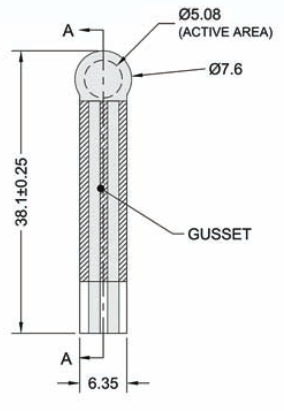
\includegraphics[width=0.3\textwidth]{obrazky-figures/fsr400.png}
	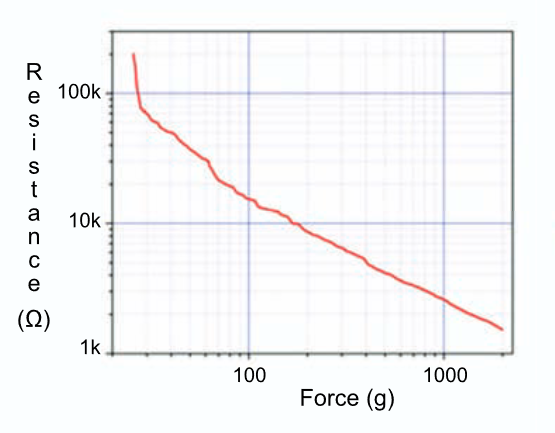
\includegraphics[width=0.5\textwidth]{obrazky-figures/FSRodporSila.png}
	\caption{Tlakový senzor FSR400 a graf vývoja odporu a sily}
	\label{Odpor sila}
\end{figure}

\begin{figure}[hbt]
	\centering
	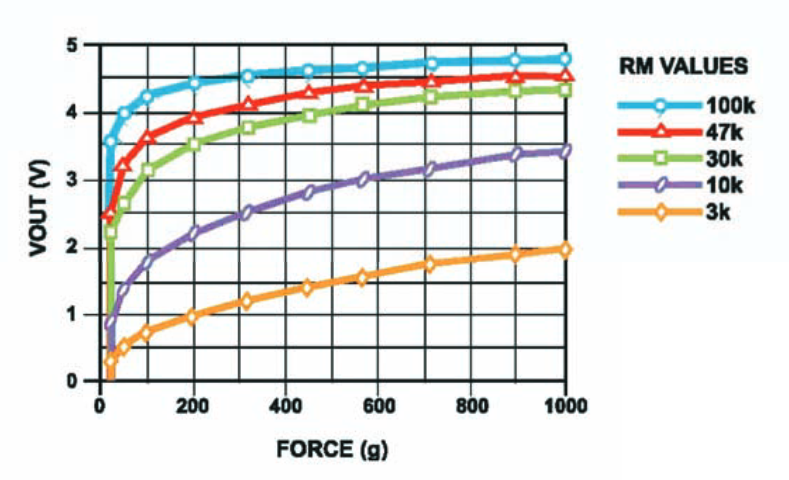
\includegraphics[width=0.6\textwidth]{obrazky-figures/fsr-charakteristikaV-force.png}
	\caption{Charakteristika elektrického napätia a sily}
	\label{Characteristics}
\end{figure}

\subsection*{Akcelerometer a akcelerometer}

Rozhodol som sa použiť modul GY-521, ktorý kombinuje obidva senzory na jednom čipe. Akcelerometre typu MEMS trpia zvýšenou hladinou šumu\cite{PawlusJan2019Zpns}, ako som sa aj ja presvedčil. Zatiaľ som mal k dispozícii len jeden modul preto som zatiaľ neotestoval použitie dvoch modulov a priemerovanie nameraných hodnôt. Ako alternatívu teraz čakám na ďalšie dva senzory DFROBOT SEN0253\cite{PohybovySenzor}, na ktorých vyskúšam priemerovanie a rôzne rozmiestnenie na pere.

\subsection*{SD karta}

Výber padol na adaptér microSD kariet DFROBOT DFR0229 kvôli jeho veľkosti a jednoduchému pripojeniu. Ako úložisko používam MicroSD kartu veľkosti 2GB. 

\subsection*{Mikrokontrolér}

Na začiatku som si vybral vývojovú dosku Arduino Nano kvôli jej jednoduchému použitiu a programovaniu. 
Počiatočné experimenty však ukázaly, že táto doska nie je vhodná, pretože jej ADC (analógovo digitálny prevodník) je príliš pomalý pri spracovávaní z viacerých senzorov. Mikrokontrolér dokázal spracovať\footnote{prečítať aktuálnu hodnotu z výstupu a zapísať ju do pamäte FLASH na SD karte} len asi 100 hodnôt za sekundu, čo je v mojom prípade málo, keže jeden podpis trvá približne do dvoch sekúnd.

Teraz som začal hľadať iný mikrokontrolér a vyskúšam vývojovú dosku ARMSTM32F103C8T6 \cite{ArduinoARM}. Tiež budem kontaktovať pána Ing. Václava Šimeka, ktorý mi hádam poradí ďalej.


\section{Návrh pera}

Rozhodol som sa pre dizajn guličkového pera, keďže zaberá menej miesta ako plniace pero. Pero bude pozostávať z niekoľkých hlavných častí - vonkajší obal, tuha, batéria a senzory spolu s ich uchytením. Vonkajší obal bude v prvotnom prototype vyrobený z plastového 10-farebného pera a plastovej trubky. Tuha bude umiestnená klasicky v strede pera. Kvôli ušetreniu miesta nepočítam so zapínacím mechanizmom a radšej som sa rozhodol pre riešenie s použitím vrchnáku, ktorý sa vyrobí v neskoršej časti vývoja a mal by pridať aj na luxusnejšom pocite z~pera. Rozhodol som sa pre kovovú tuhu do guličkového pera, pretože som si vybral tlakový odporový senzor a potrebujem aby tuha nebola flexibilná. 

\subsubsection*{Uchytenie tlakových senzorov}

Na uchytenie tlakových senzorov bude použitý prstenec s prítlačnými "stavěcími skrutkami" s plastovou dosadacou plochou valcového tvaru s priemerom $\phi$~3mm. Dookola 

\begin{figure}[hbt]
	\centering
	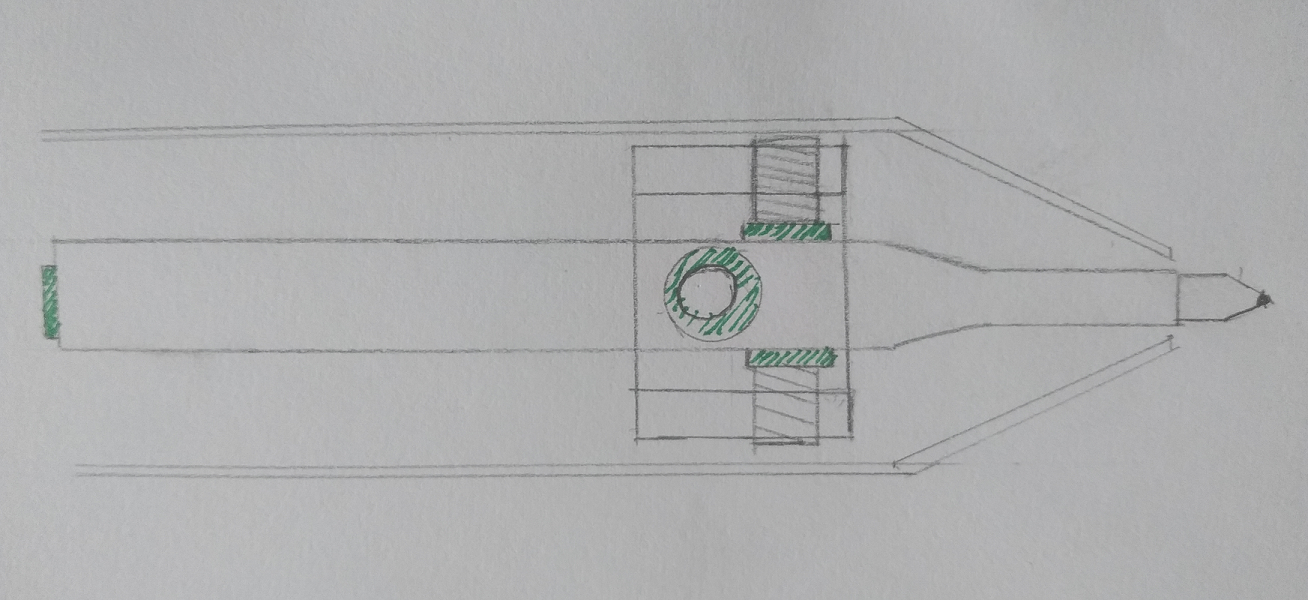
\includegraphics[width=0.4\textwidth]{obrazky-figures/umiestnenie_tlakovych_senzorov.png}
	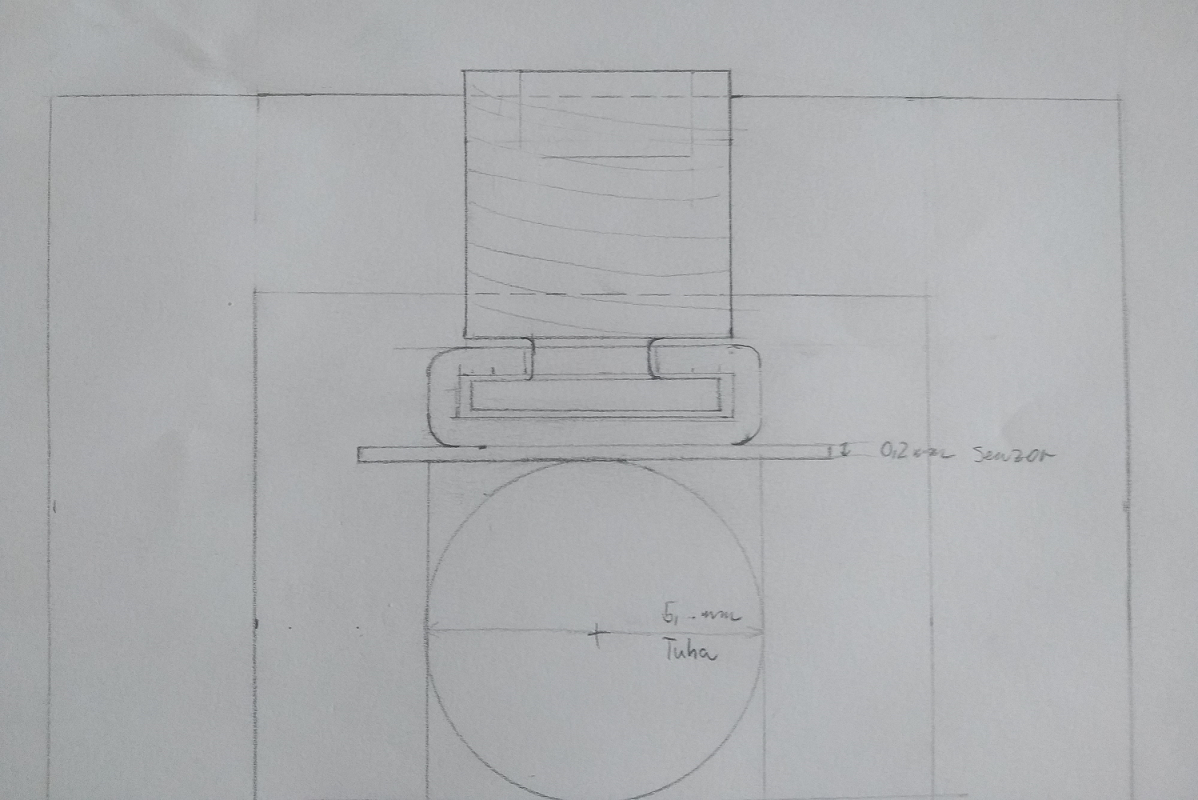
\includegraphics[width=0.4\textwidth]{obrazky-figures/uchytenie.png}
	\caption{Návrh uchytenia tuhy (vľavo) a uchytenie tlakového senzora (vpravo)}
	\label{Uchytenie tuhy}
\end{figure}

Keď chceme určiť akou vzorkovacou frekvenciou chceme analógové hodnoty tlaku na hrot čítať potrebujeme vedieť čas a dĺžku napísaného textu. Ak sa zamyslíme pri akej príležitosti človek vykoná najrýchlejší pohyb rukou, tak nám jednoznačne napadne podpisovanie. Pri podpisovaní človek robí automatizovaný pohyb, ktorý má proste "v ruke" (z angličtiny muscle memory). Urobil som experiment na niekoľkých subjektoch, ktorým som nepovedal, čo meriam a nechal som ich podpísať sa. Odstopoval som koľko im trvalo ich bežné podpísanie a hodnoty som si zaznamenal. Toto testovanie prebiehalo na malej vzorke 10 ľudí a jeho cieľom bolo nájsť najrýchlejší podpis - keďže by sme chceli, aby pero dokázalo pracovať aj v náročných podmienkach. Potreboval som len referenčnú hodnotu podľa ktorej by som vedel vybrať vhodný mikrokontrolér s vhodným A/D prevodníkom. 

Tento experiment by sa mohol vylepšiť použitím pera s jedným tlakovým senzorom, ktorý by si pri začiatku podpisu zaznamenal čas a pri detekovaní tlaku by zaznamenal úvodný čas a na konci by zaznamenal koncový čas. Takto by sme dostali presnejšie hodnoty.

Experimentálne sme zistili, že najrýchlejší podpis trvá len 0.8 s, pričom nevylučujeme možnosť rýchlejšieho podpisu. Ak budeme chcieť vzorkovať podpis povedzme po 1 mm musíme zmerať dĺžku podpisu. v tomto prípade sa jednalo o dĺžku asi 60 mm. Ak si to prevedieme trojčlenkou výjde nám, že za 1 sekundu urobí 75 mm a teda potrebujeme 75 vzorkov za sekundu - 75 Hz. Experimentálna vzorkovacia frekvencia vo výskume z roku 1990\cite{SchomakerL.1990Trbp} bola 105 Hz pričom rozlíšenie bolo nastavené na 0.025 mm s presnosťou 0.25 mm. Z tohoto dôvodu nastavíme aj my vzorkovaciu frekvenciu na hodnotu 100 Hz.

\section{Nepoužité komponenty}

V tejto časti v skratke popíšem, ktoré súčiastky by sa mohli použiť v ďaľích prototypoch.

Mikrofón by sa mohol použiť ako senzor pre zachytenie širšieho kontextu, podobne ako to má Livescribe 3. Vedeli by sme potom k čomu sa písaný text viaže alebo aký dokument sa podpisuje. 

Ak by sme chceli merať ďalšie biometrické dáta mohli by sme použiť merač tepu na miestach kde sa človek dotýka pera. Ak bude osoba písať dlhší text vedeli by sme zistiť nakoľko je nervózna. 

Použitie bezdrôtového pripojenia, napr. BLE (Bluetooth Low Energy) by uľahčilo získavanie dát z pera, keďže ak sa chceme dostať k informáciám na SD karte musíme pero rozobrať. Toto riešnie by mohlo aj zmenšiť rozmery pera.

\chapter{Realizace řešení}

\section{Experimenty}

\subsection*{Testovanie súčiatok}

\begin{figure}[hbt]
	\centering
	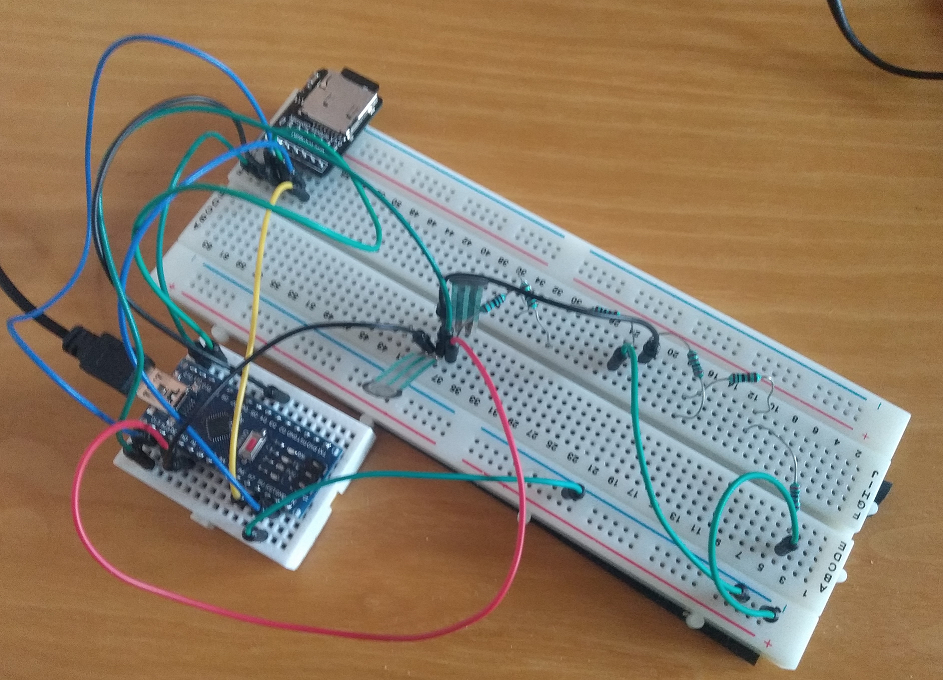
\includegraphics[width=0.5\textwidth]{obrazky-figures/FSRtestSD.png}
	\caption{Ukladanie dát na pamäťovú kartu}
	\label{Experiment1}
\end{figure}

\section{vyhodnocení výsledů}

\chapter{Závěr}

\label{zaver}

%===============================================================================
